\chapter{Architecture Overview}

The Architecture Overview chapter is designed to give you a basic
understanding of each of the Gravwell components, how Gravwell models
data, how data flows through Gravwell, and the different ways in which
Gravwell can be deployed. We will examine a few basic deployments,
gradually increasing in capacity and complexity. Gravwell is designed
to be able to scale to many hundreds of nodes, but it can just as easily
run in a container, with all the services coexisting on a minimal system.

\section{Terminology}

Gravwell is a large system with quite a few moving parts. It is
important to start by establishing some terminology so that everyone can
speak the same language.

\begin{description}[font=\sffamily\bfseries, leftmargin=1cm, style=nextline]
\item[Indexer]\index{Indexers}
Stores data and manages wells.

\item[Webserver]\index{Webservers}
Serves web interface, controls and coordinates indexers.

\item[Entry]\index{Entries}
A single tagged record or data item (line from a log file, Windows event, packet, etc.)

\item[Enumerated Value]\index{Enumerated Values}
Named data item that is extracted from the raw entry during a search.

\item[Tag]\index{Tags}
Human-readable name for a data group. The most basic grouping of data.

\item[Well]\index{Wells}
On-disk collection of entries. Every entry ends up in exactly one well, sorted by tag.

\item[Shard]\index{Shards}
A slice of data within a well. Each shard contains about 1.5 days of entries.

\item[Ingester]\index{Ingesters}
Program that accepts raw data and packages it as entries for transport to an indexer.

\item[Renderer]\index{Search!renderers}\index{Renderers}
Query component that collects search output and presents results to a human.

\item[Datastore]\index{Datastore}
Central authority of users and user-owned objects for distributed webservers.

\item[Search Agent]\index{Search agent}
Monitors and launches automated queries and scripts on behalf of users.

\item[Cluster Deployment]\index{Clusters}
Multiple Indexers all participating in a single Gravwell instance.

\item[Distributed Webservers]\index{Distributed webservers}
Multiple webservers sharing the load of GUI interactions and queries, but controlling the same set of indexers.

\item[Load Balancer]\index{Load balancer}
An HTTP reverse proxy which transparently balances load across multiple webservers.
\end{description}

\section{Gravwell Entries}

Gravwell stores all data as \emph{entries}\index{Entries}. An entry consists of a piece of data (just an array of bytes), a timestamp, a tag, and a source address. Each of these components deserves a bit of explanation, so we will cover each separately. Entries are stored in an efficient binary format on disk, but a user-friendly representation of an example entry would look something like this:

\begin{Verbatim}[breaklines=true]
{
    Data: `127.0.0.1 - frank [10/Oct/2000:13:55:36 -0700] 
"GET /apache_pb.gif HTTP/1.0" 200 2326 "http://www.example.com/start.html" 
"Mozilla/4.08 [en] (Win98; I ;Nav)"`,
    Timestamp: 2000-10-10 13:55:36 -0700 MST,
    Tag: "apache-logs",
    Source: 10.0.2.3,
}
\end{Verbatim}

\subsection{``Timestamp'' field}

The timestamp\index{Timestamps} is meant to indicate the creation time of the \emph{data}. This is typically extracted from the data itself by the ingester, e.g. by parsing out the timestamps on syslog messages. However, some ingesters such as the packet logger will instead set the timestamp to the current time, since the packet was captured ``now''.

\subsection{``Data'' field}

The data field contains the actual raw data of the entry. If log files are being ingested, the data field will typically contain a single line from the log file. When ingesting network packets, the data field will contain a single binary packet.

\subsection{``Tag'' field}

The tag\index{Tags} field categorizes the entry. Users refer to tags by strings, e.g. ``default'' or ``pcap'' or ``windows-logs'', but under the hood Gravwell assigns each tag string a unique numeric ID for more efficient storage.

\subsection{``Source'' field}

The source\index{SRC|see {Source}}\index{Source} field indicates where the entry originated. It is an IPv4 or IPv6 address. It is perhaps the most free-form field of the entry, because it can indicate the machine on which the ingester was located, the machine from which the ingester \emph{read} the entry data, or it can be an entirely arbitrary number chosen as a second layer of categorization beyond the tag. Most ingesters provide configuration options for how the source field should be set.

\clearpage
\section{Data Ingest}

A core function of Gravwell is data ingest\index{Data ingest}; \emph{ingesters}\index{Ingesters} take raw data, package it as entries,
and transmit those entries to a Gravwell indexer (or
indexers) for storage, indexing, and searching. The Gravwell
ingest API\footnote{https://github.com/gravwell/gravwell/tree/master/ingest}
is open source and so are most of the core
ingesters\footnote{https://github.com/gravwell/gravwell/tree/master/ingesters}.  Ingesters can
often feed from multiple data sources at once, and each ingester may
upload its entries to a single indexer or multiple indexers.


\begin{figure}
	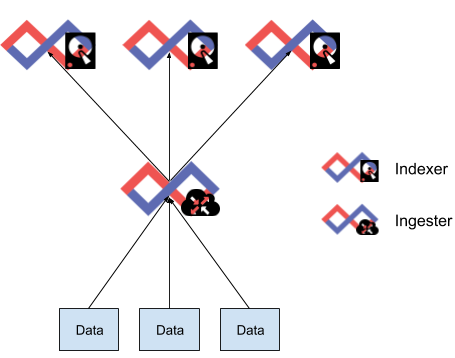
\includegraphics[width=0.6\linewidth]{images/dataingest.png}
	\caption{Data Ingest}
\end{figure}

Here are some key concepts for ingesters:


\begin{enumerate}
\tightlist
\item
  {Ingesters are separate from indexers.}
\item
  {Ingesters may run on remote systems.}
\item
  {Ingesters send entries to indexers.}
\item
  {Ingesters assign tags to entries.}
\item
  {Ingesters can create new tags.}
\item
  {Ingesters can cache entries locally if an indexer is not available.}
\item
  {Ingesters can multiplex across many indexers.}
\item
  {Ingesters can throttle their entry upload rate.}
\item
  {Ingesters authenticate with indexers via a secure challenge-response protocol.}
\item
  {Authentication is secure over a cleartext connection.}
\item
  {Entry transmission is \emph{only} secure when operating over a validated TLS
  connection with valid TLS certificates.}
\end{enumerate}

An entry represents an atomic thing in gravwell whether that be a
packet, log line, or binary blob. Entries always contain four fields:
timestamp, tag, source, data. The ingesters are responsible for setting
those fields.

Entry timestamps are independent of the raw data, although they may be
derived from the raw data. For example, an ingester may detect the
timestamp in an Apache log line and apply it to the entry, or it may
apply the current timestamp.

For more information about available
Gravwell ingesters, visit the Gravwell documentation site at
{\href{https://docs.gravwell.io}{https://docs.gravwell.io}

\clearpage
\section{Example Gravwell Deployments}

Gravwell can be deployed on a single node, a cluster of indexers and one webserver, a
cluster of indexers and a cluster of webservers, or even as geographically-dispersed subclusters.
Users interact with Gravwell using either a standards-compliant browser
(we like Chromium and Firefox) or the provided Gravwell command line
interface. For each deployment example we will show some basic diagrams
which will use the icons in Figure \ref{fig:archicons} to depict each component.

\begin{figure}
	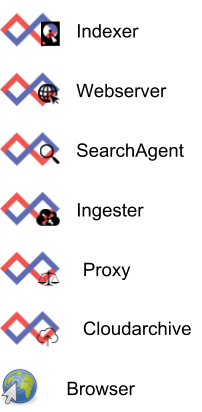
\includegraphics[width=0.2\linewidth]{images/archicons.png}
	\caption{Icons used}
	\label{fig:archicons}
\end{figure}

\subsection{Single Node}

The simplest Gravwell deployment topology is a single node where all
components are co-resident on a single host or container. When
operating in a single node deployment, Gravwell optimizes queries to
maintain data locality. This means that webserver participation in the
query pipeline is minimal, typically only running the renderer module.
The complete Gravwell deployment contains three core components (Indexer,
Webserver, and Search Agent), plus any number of ingesters (both on and off the node) as shown in Figure \ref{fig:singlenode}.

\begin{figure}
	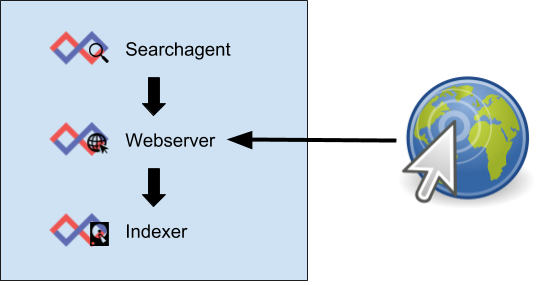
\includegraphics[width=0.6\linewidth]{images/singlenode.png}
	\caption{Single-node deployment}
	\label{fig:singlenode}
\end{figure}


\subsection{Cluster Deployment}

Gravwell deployments that need to handle large data volumes may require
multiple indexers. A Gravwell cluster\index{Clusters} is comprised of multiple indexers
which are controlled by a single webserver as shown in Figure \ref{fig:cluster}. The webserver and
search agent are typically on a separate node and connect to the indexers
via an IPv4 or IPv6 link. When operating in a cluster topology Gravwell
will intelligently break up and distribute a query so that as much of
the query pipeline as possible runs on the indexers, condensing
the pipeline to the webserver only when necessary. Depending on the
query, cluster topologies may transmit significant data volumes between
the indexers and webserver, so it is important that the links between
the webservers and indexers be fast, with low latencies and high
bandwidth. While it is possible to geographically separate a webserver
from an indexer over a WAN link, the increased latency and decreased
bandwidth will affect query performance.

\begin{figure}
	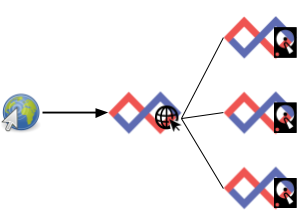
\includegraphics[width=0.6\linewidth]{images/cluster.png}
	\caption{Cluster Deployment}
	\label{fig:cluster}
\end{figure}

\subsection{Distributed Webserver Architecture}

Very large Gravwell deployments with many users may need to also employ
multiple webservers\index{Distributed webservers} to handle the load. Gravwell supports a distributed
webserver topology by coordinating and synchronizing the webservers, 
shown in Figure \ref{fig:distributed}.

\begin{figure}
	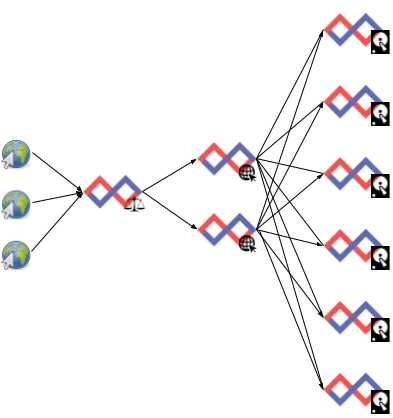
\includegraphics[width=0.6\linewidth]{images/distributed.png}
	\caption{Distributed Webserver Architecture}
	\label{fig:distributed}
\end{figure}

Webservers coordinate and synchronize using a component called the
\emph{datastore}\index{Datastore}. The datastore acts as a master storage system for user data,
search resources, scheduled queries, scripts, and any other component
that can be uploaded or modified by a user. Webservers and the
datastore will attempt to maintain a complete copy of all resources,
which allows webservers to fail and be restored by simply rejoining the
cluster. However, the datastore is treated as the master copy, so while
the datastore component requires minimal CPU resources, robust storage is advised.

\clearpage
\section{Replication}

Gravwell supports full data replication\index{Replication}, so that in the event of
hardware failure, data is not lost. Replication strategies depend on
the type of deployment and general tolerance for distributed failures.
Replication is controlled entirely by the indexers and is unaffected by
the webserver deployment. Gravwell supports two forms of replication:
online and offline.

\subsection{Online Replication}

Online replication requires that indexers communicate directly with one
another and coordinate data replication. Online replication provides
hot-failover, meaning that if an indexer fails the other indexers in the
replication group will detect the failure and serve the failed node's
data during a query.

\begin{figure}
	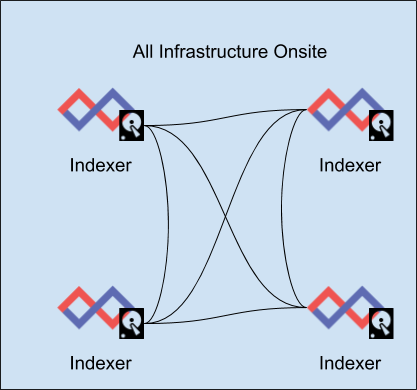
\includegraphics[width=0.6\linewidth]{images/onlinereplication.png}	
	\caption{Online Replication}
	\label{fig:onlinereplication}
\end{figure}


\subsection{Offline Replication}

Offline replication is achieved using a dedicated replication component
which does not participate in queries. Indexers will replicate their
data to the offline replication service and only pull data back in the
event of a failure. A single offline replicator may service many
indexers (provided that it has adequate storage). The offline
replicator can be onsite or offsite.

\begin{figure}
	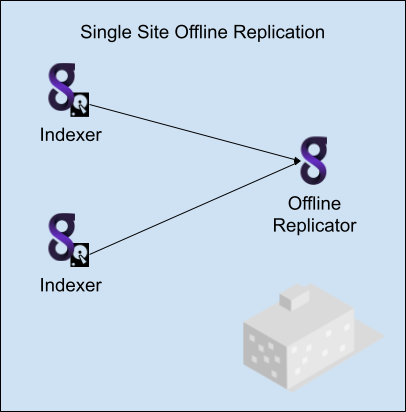
\includegraphics[width=0.6\linewidth]{images/offlinereplication.png}
	\caption{Offline Replication}
	\label{fig:offlinereplication}
\end{figure}

\section{Scheduled Search and Orchestration}

Gravwell includes an automated search and scripting system. Using
scheduled searches and scripts you can keep resources up to date, export
data, run multiple queries and alert on the results, or even take action
on remote systems based on the results of a query. The scheduled search
and orchestration scripts are executed by the search agent. The search agent
is a standalone component which communicates with one or more webservers
and invokes queries and scripts as needed, as shown in Figure \ref{fig:scheduledsearch}. 
There is only ever one
search agent in a deployment, and the default Gravwell deployment
colocates the searchagent with the webserver. However, in a distributed
webserver topology the search agent may be located on its own node.

\begin{figure}
	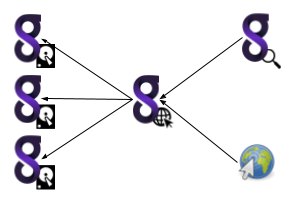
\includegraphics[width=0.6\linewidth]{images/soar.png}
	\caption{Scheduled Search and Orchestration}
	\label{fig:scheduledsearch}
\end{figure}
